\documentclass[aspectratio=169,10pt]{beamer}

\usetheme{Madrid}
\usecolortheme{default}
\setbeamertemplate{navigation symbols}{}
\setbeamertemplate{footline}[frame number]

\usepackage[T1]{fontenc}
\usepackage[utf8]{inputenc}
\usepackage{amsmath,amssymb}
\usepackage{booktabs}
\usepackage{array}
\usepackage{graphicx}
\usepackage{tikz}
\usetikzlibrary{arrows.meta,positioning,fit,calc,shapes.geometric}
\usepackage{pgfplots}
\pgfplotsset{compat=1.18}

\title[Fairness-Aware Routing]{Fairness-Aware Routing Under Missing Context}
\subtitle{Clinical and Quantum Sequential Decision Systems with MAB, CMAB, and iCMAB Methods}
\author[P. Z. Garcia Bautista]{Piter Z. Garcia Bautista\\Advisors: Daniel Krutz and Travis Desell}
\institute[RIT]{Rochester Institute of Technology\\DSCI 601 -- Applied Data Science I}
\date{Endterm Presentation}

\definecolor{ritorange}{RGB}{247,105,2}
\definecolor{deepblue}{RGB}{31,78,121}
\definecolor{softgreen}{RGB}{72,160,98}
\definecolor{softred}{RGB}{190,75,72}
\definecolor{softgray}{RGB}{245,247,250}
\definecolor{softblue}{RGB}{88,137,174}
\definecolor{softpurple}{RGB}{135,99,171}

\setbeamercolor{title}{fg=deepblue}
\setbeamercolor{frametitle}{fg=deepblue}
\setbeamercolor{structure}{fg=ritorange}

\newcommand{\mab}{\textsc{MAB}}
\newcommand{\cmab}{\textsc{CMAB}}
\newcommand{\icmab}{\textsc{iCMAB}}
\newcommand{\sds}{\textsc{SDS}}
\newcommand{\equitas}{\textsc{EQUITAS}}

% Compile from the presentation/ directory.
% Figures live in presentation/analysis_artifacts/.
\newcommand{\routingfig}{%
\IfFileExists{analysis_artifacts/fig1_routing_network.png}{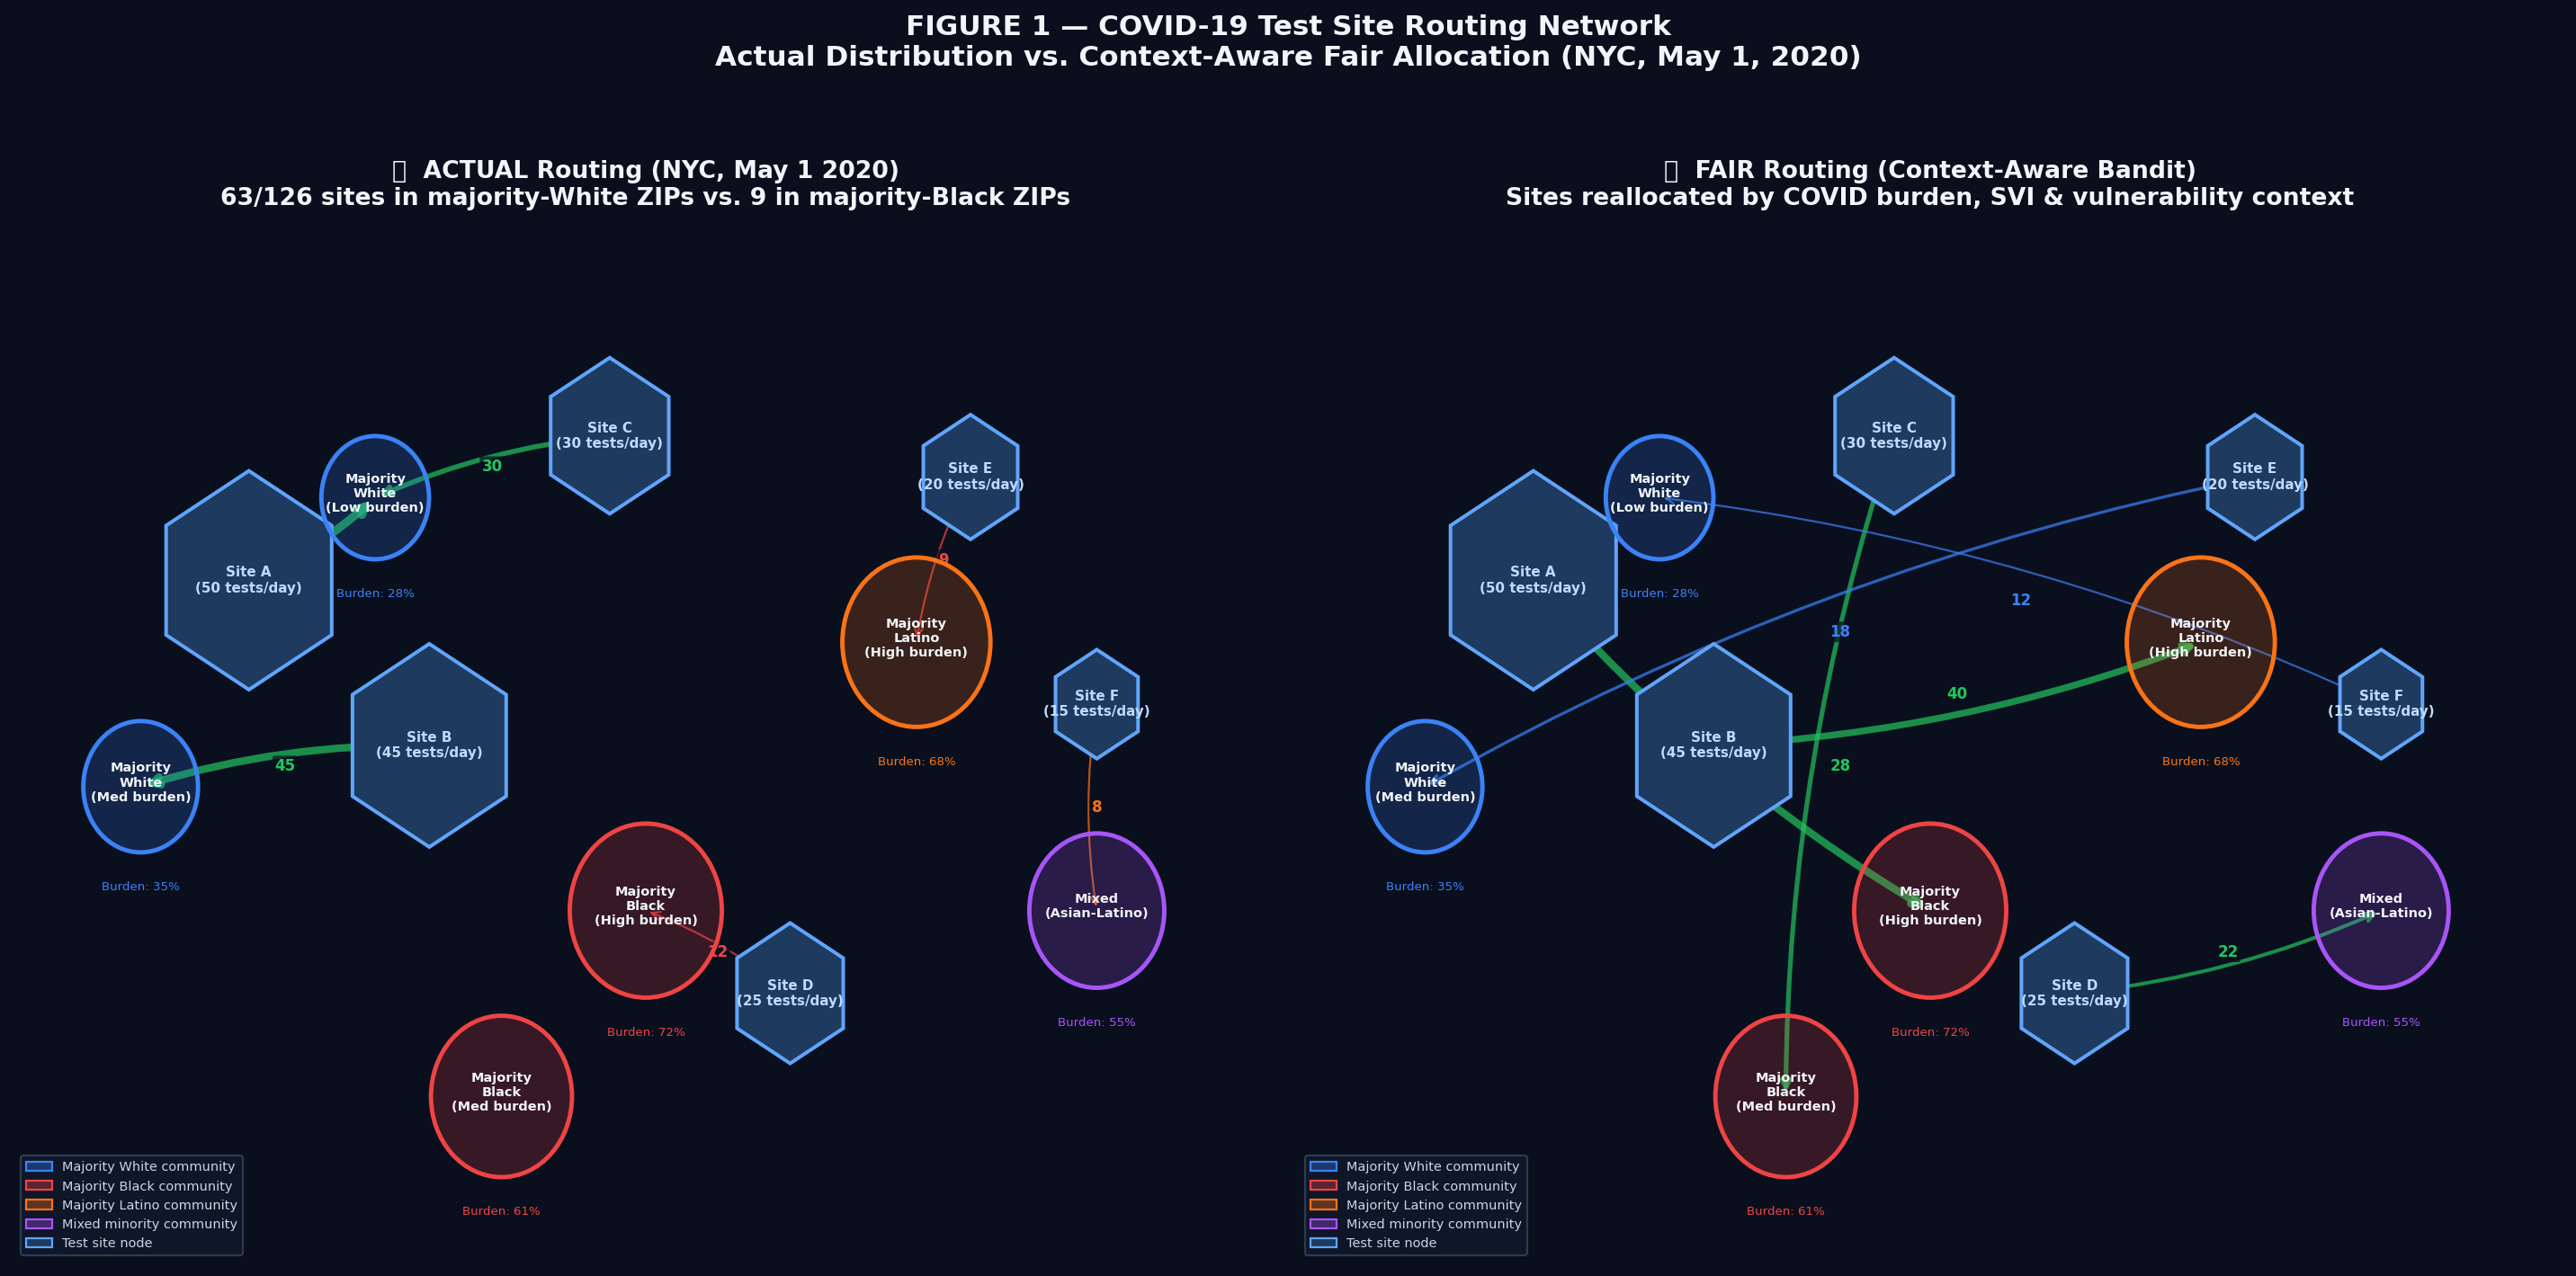
\includegraphics[width=\textwidth,height=0.68\textheight,keepaspectratio]{analysis_artifacts/fig1_routing_network.png}}{%
\IfFileExists{analysis_artifacts/graph1_routing.png}{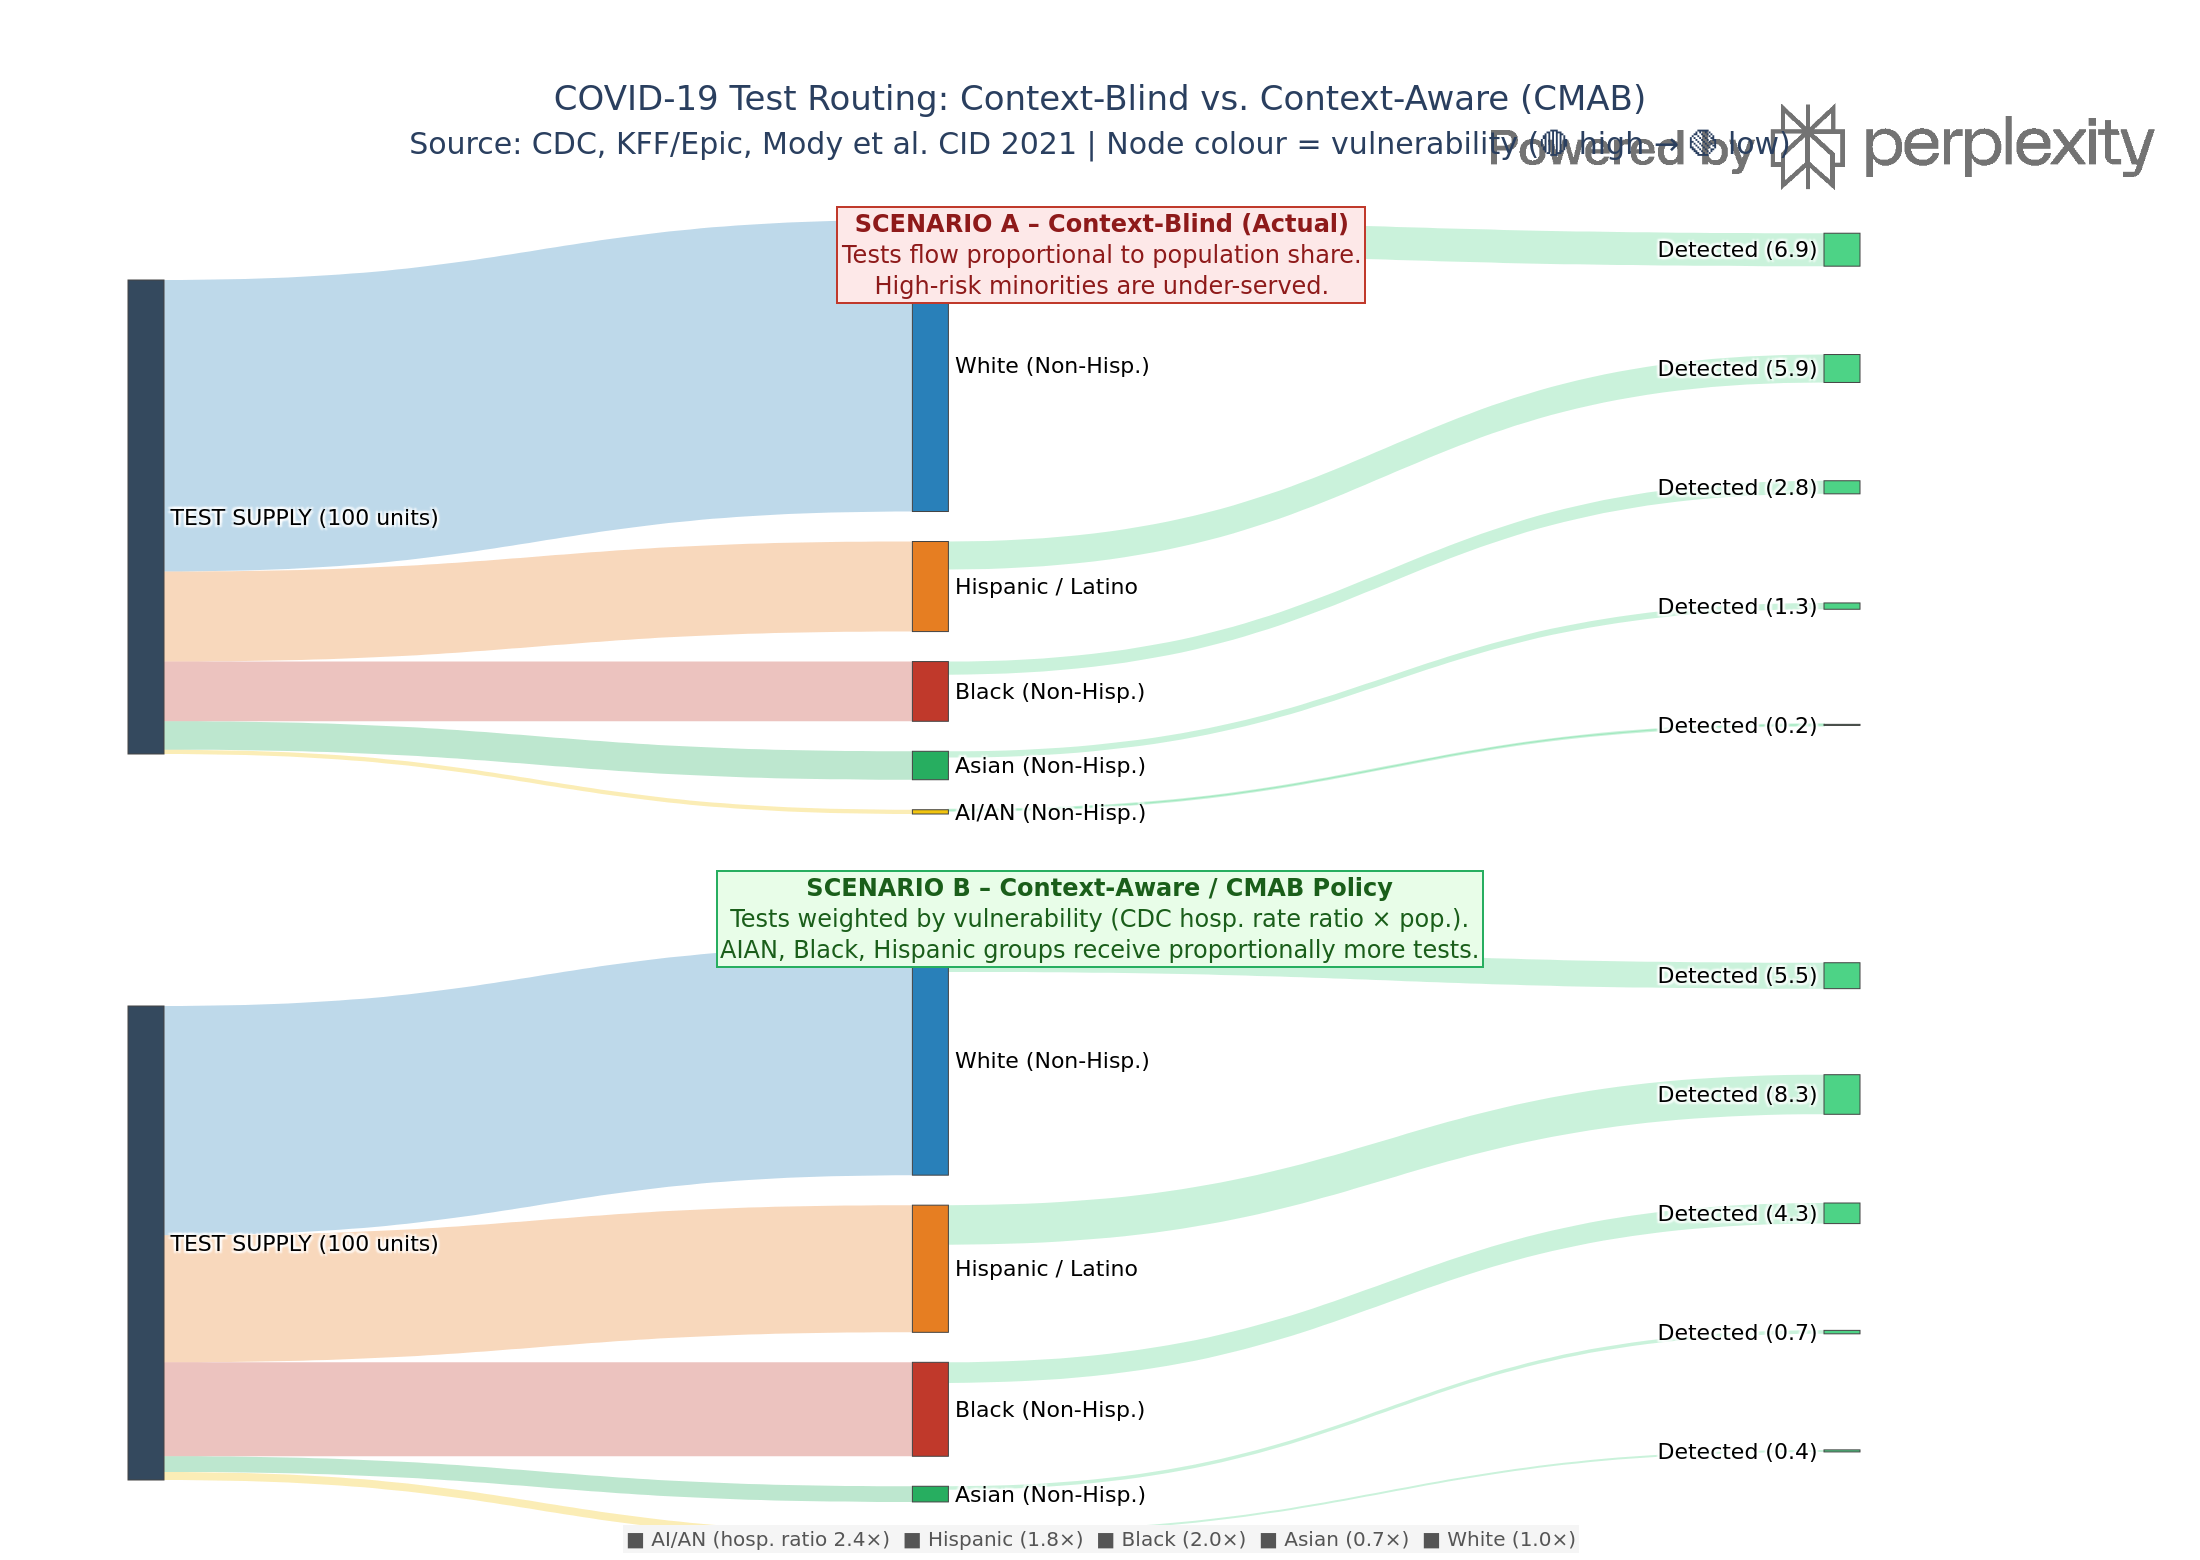
\includegraphics[width=\textwidth,height=0.68\textheight,keepaspectratio]{analysis_artifacts/graph1_routing.png}}{%
\IfFileExists{analysis_artifacts/graph1_context_blind_vs_cmab.png}{\includegraphics[width=\textwidth,height=0.68\textheight,keepaspectratio]{analysis_artifacts/graph1_context_blind_vs_cmab.png}}{%
\IfFileExists{analysis_artifacts/inefficient_test_routing.png}{\includegraphics[width=\textwidth,height=0.68\textheight,keepaspectratio]{analysis_artifacts/inefficient_test_routing.png}}{%
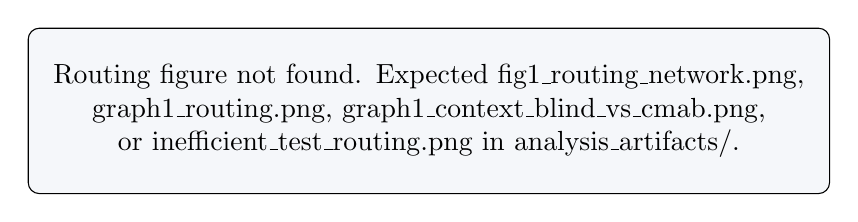
\begin{tikzpicture}\node[draw,rounded corners,fill=softgray,text width=0.82\textwidth,align=center,minimum height=2.1cm]{Routing figure not found. Expected fig1\_routing\_network.png, graph1\_routing.png, graph1\_context\_blind\_vs\_cmab.png, or inefficient\_test\_routing.png in analysis\_artifacts/.};\end{tikzpicture}}}}}}

\newcommand{\diagnosticfig}{%
\IfFileExists{analysis_artifacts/fig2_trial_bias.png}{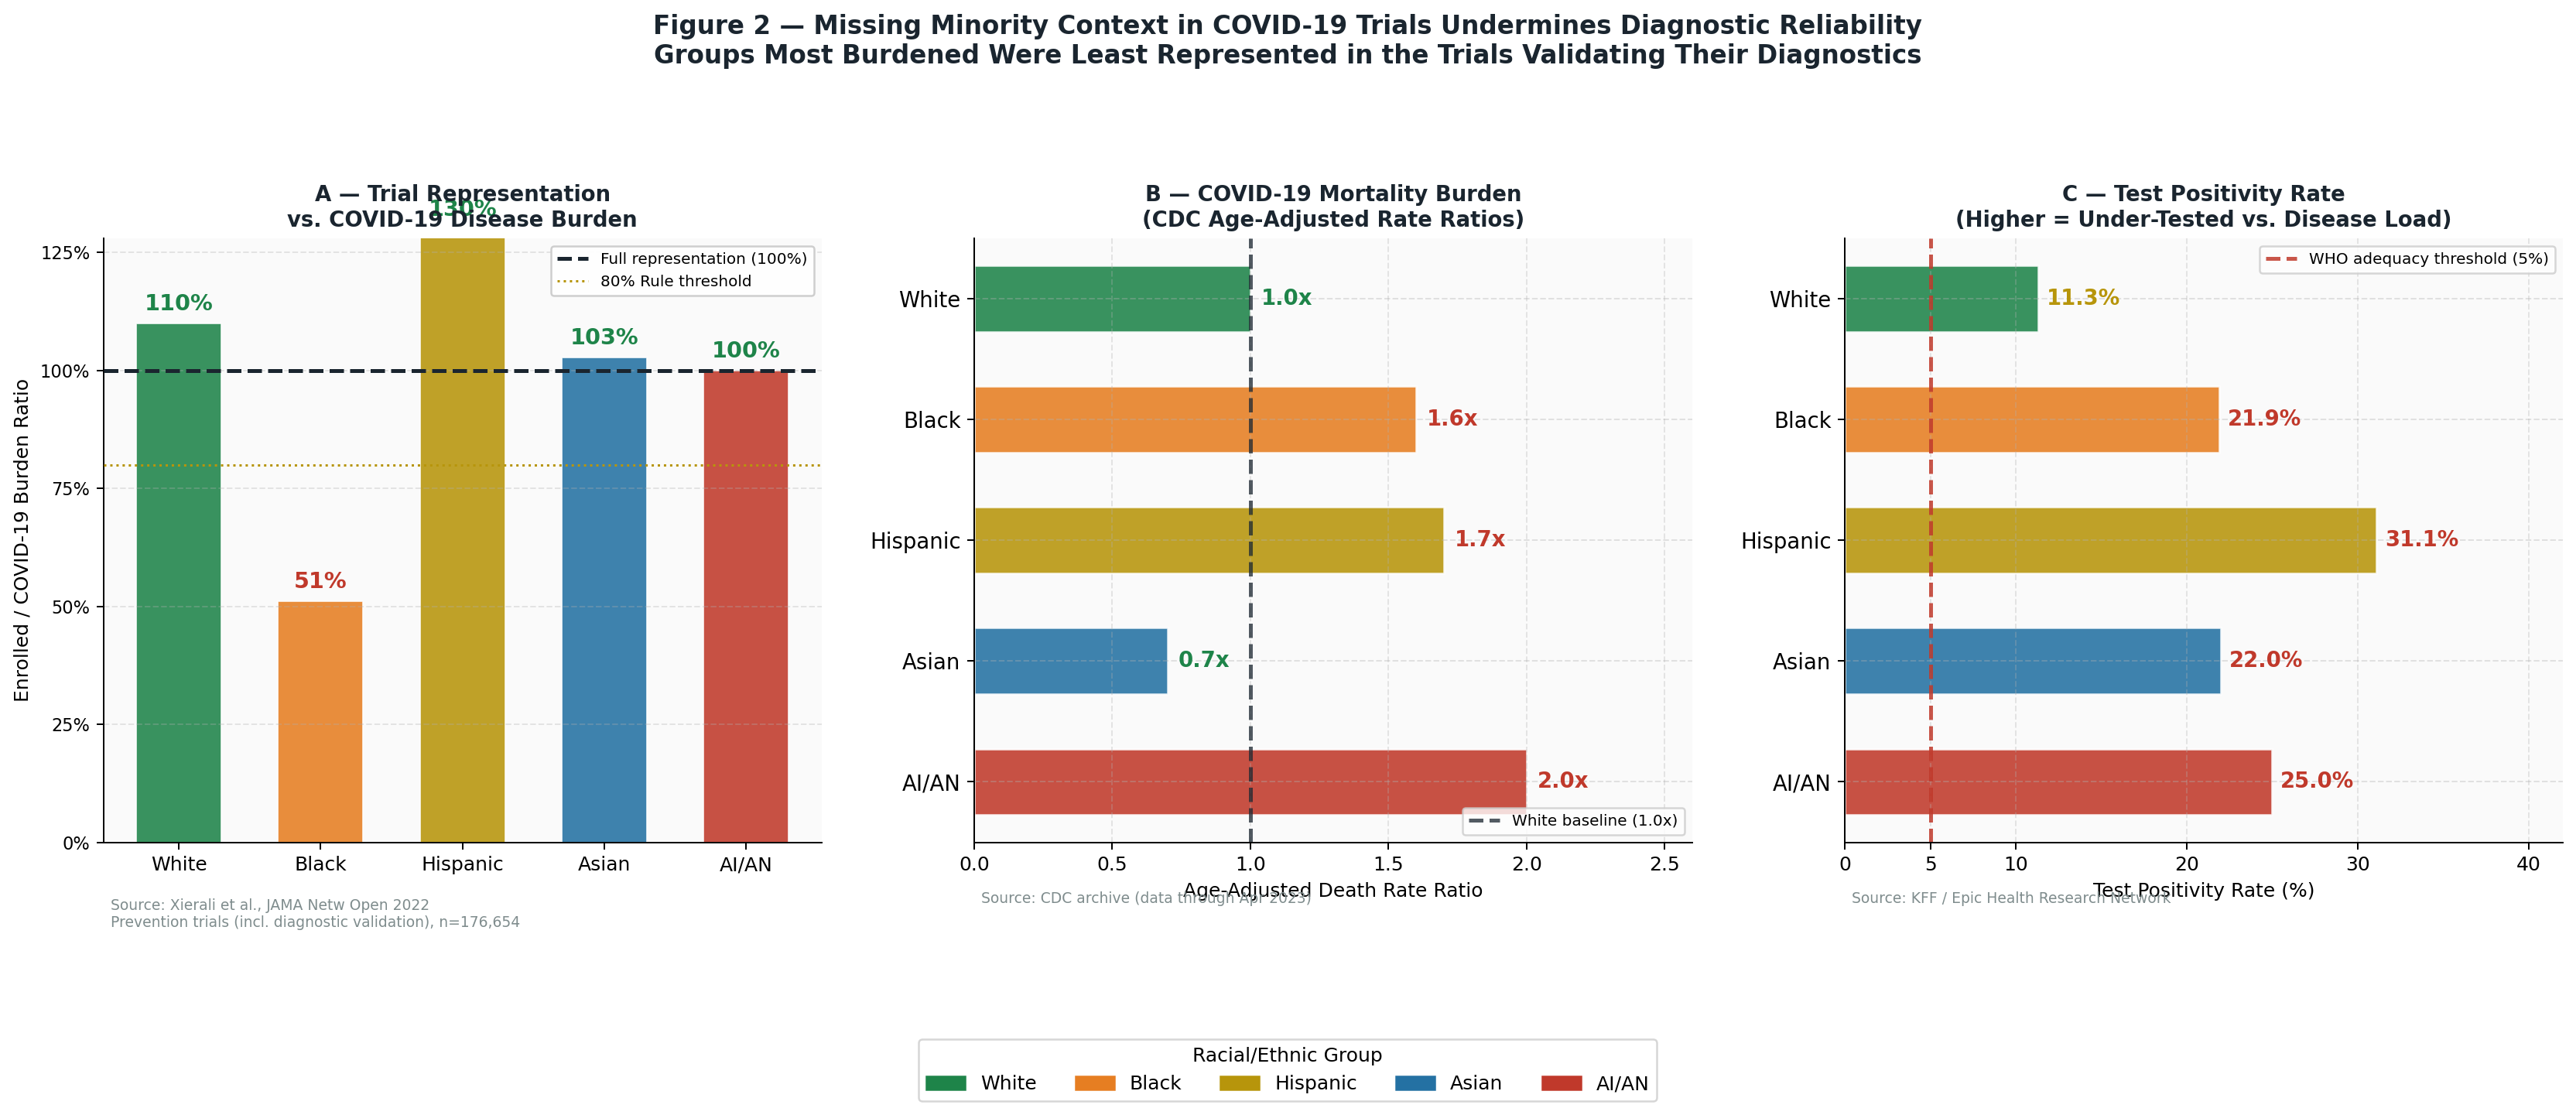
\includegraphics[width=\textwidth,height=0.68\textheight,keepaspectratio]{analysis_artifacts/fig2_trial_bias.png}}{%
\IfFileExists{analysis_artifacts/graph2_trial_bias.png}{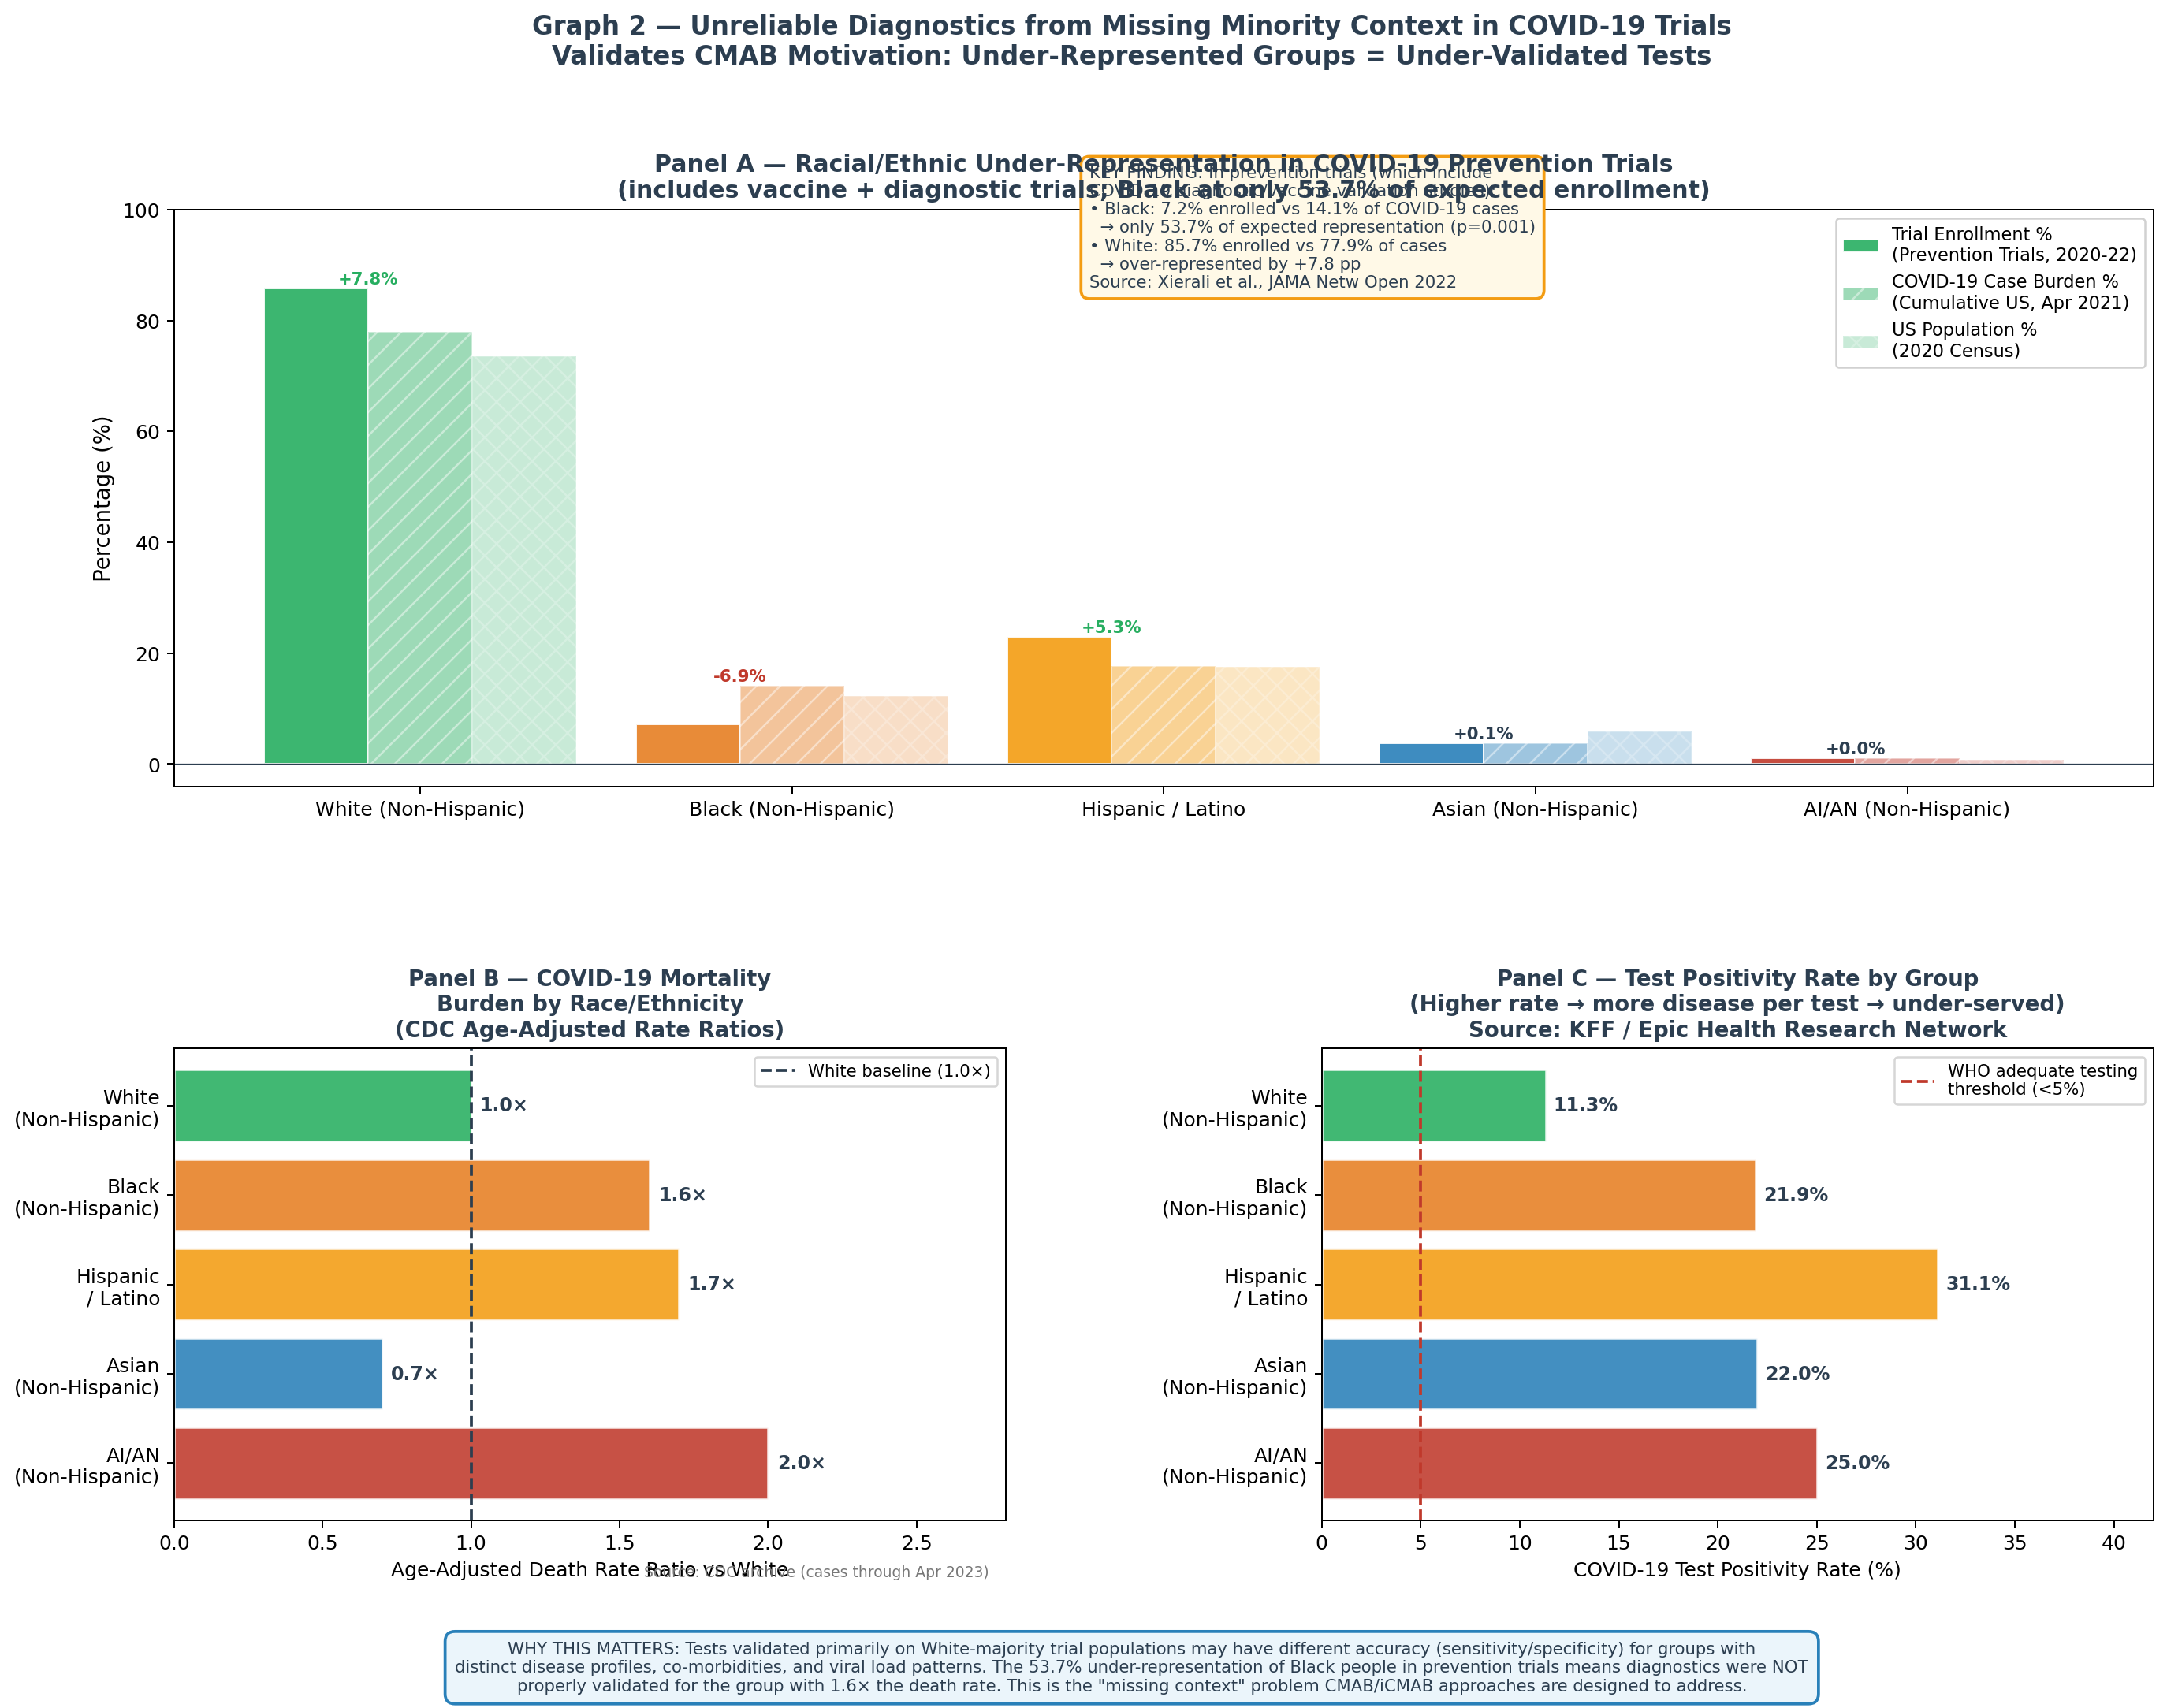
\includegraphics[width=\textwidth,height=0.68\textheight,keepaspectratio]{analysis_artifacts/graph2_trial_bias.png}}{%
\IfFileExists{analysis_artifacts/graph2_unreliable_diagnostics.png}{\includegraphics[width=\textwidth,height=0.68\textheight,keepaspectratio]{analysis_artifacts/graph2_unreliable_diagnostics.png}}{%
\IfFileExists{analysis_artifacts/unreliable_diagnostics_missing_context.png}{\includegraphics[width=\textwidth,height=0.68\textheight,keepaspectratio]{analysis_artifacts/unreliable_diagnostics_missing_context.png}}{%
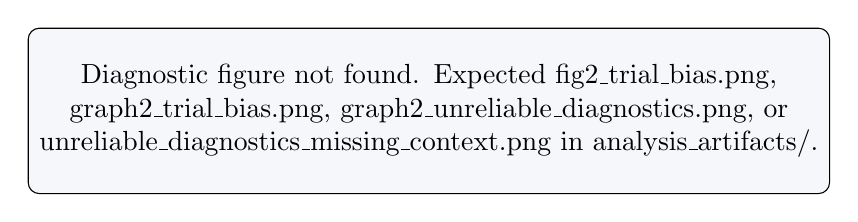
\begin{tikzpicture}\node[draw,rounded corners,fill=softgray,text width=0.82\textwidth,align=center,minimum height=2.1cm]{Diagnostic figure not found. Expected fig2\_trial\_bias.png, graph2\_trial\_bias.png, graph2\_unreliable\_diagnostics.png, or unreliable\_diagnostics\_missing\_context.png in analysis\_artifacts/.};\end{tikzpicture}}}}}}

\newcommand{\confusionfig}{%
\IfFileExists{analysis_artifacts/fig3_confusion_matrices.png}{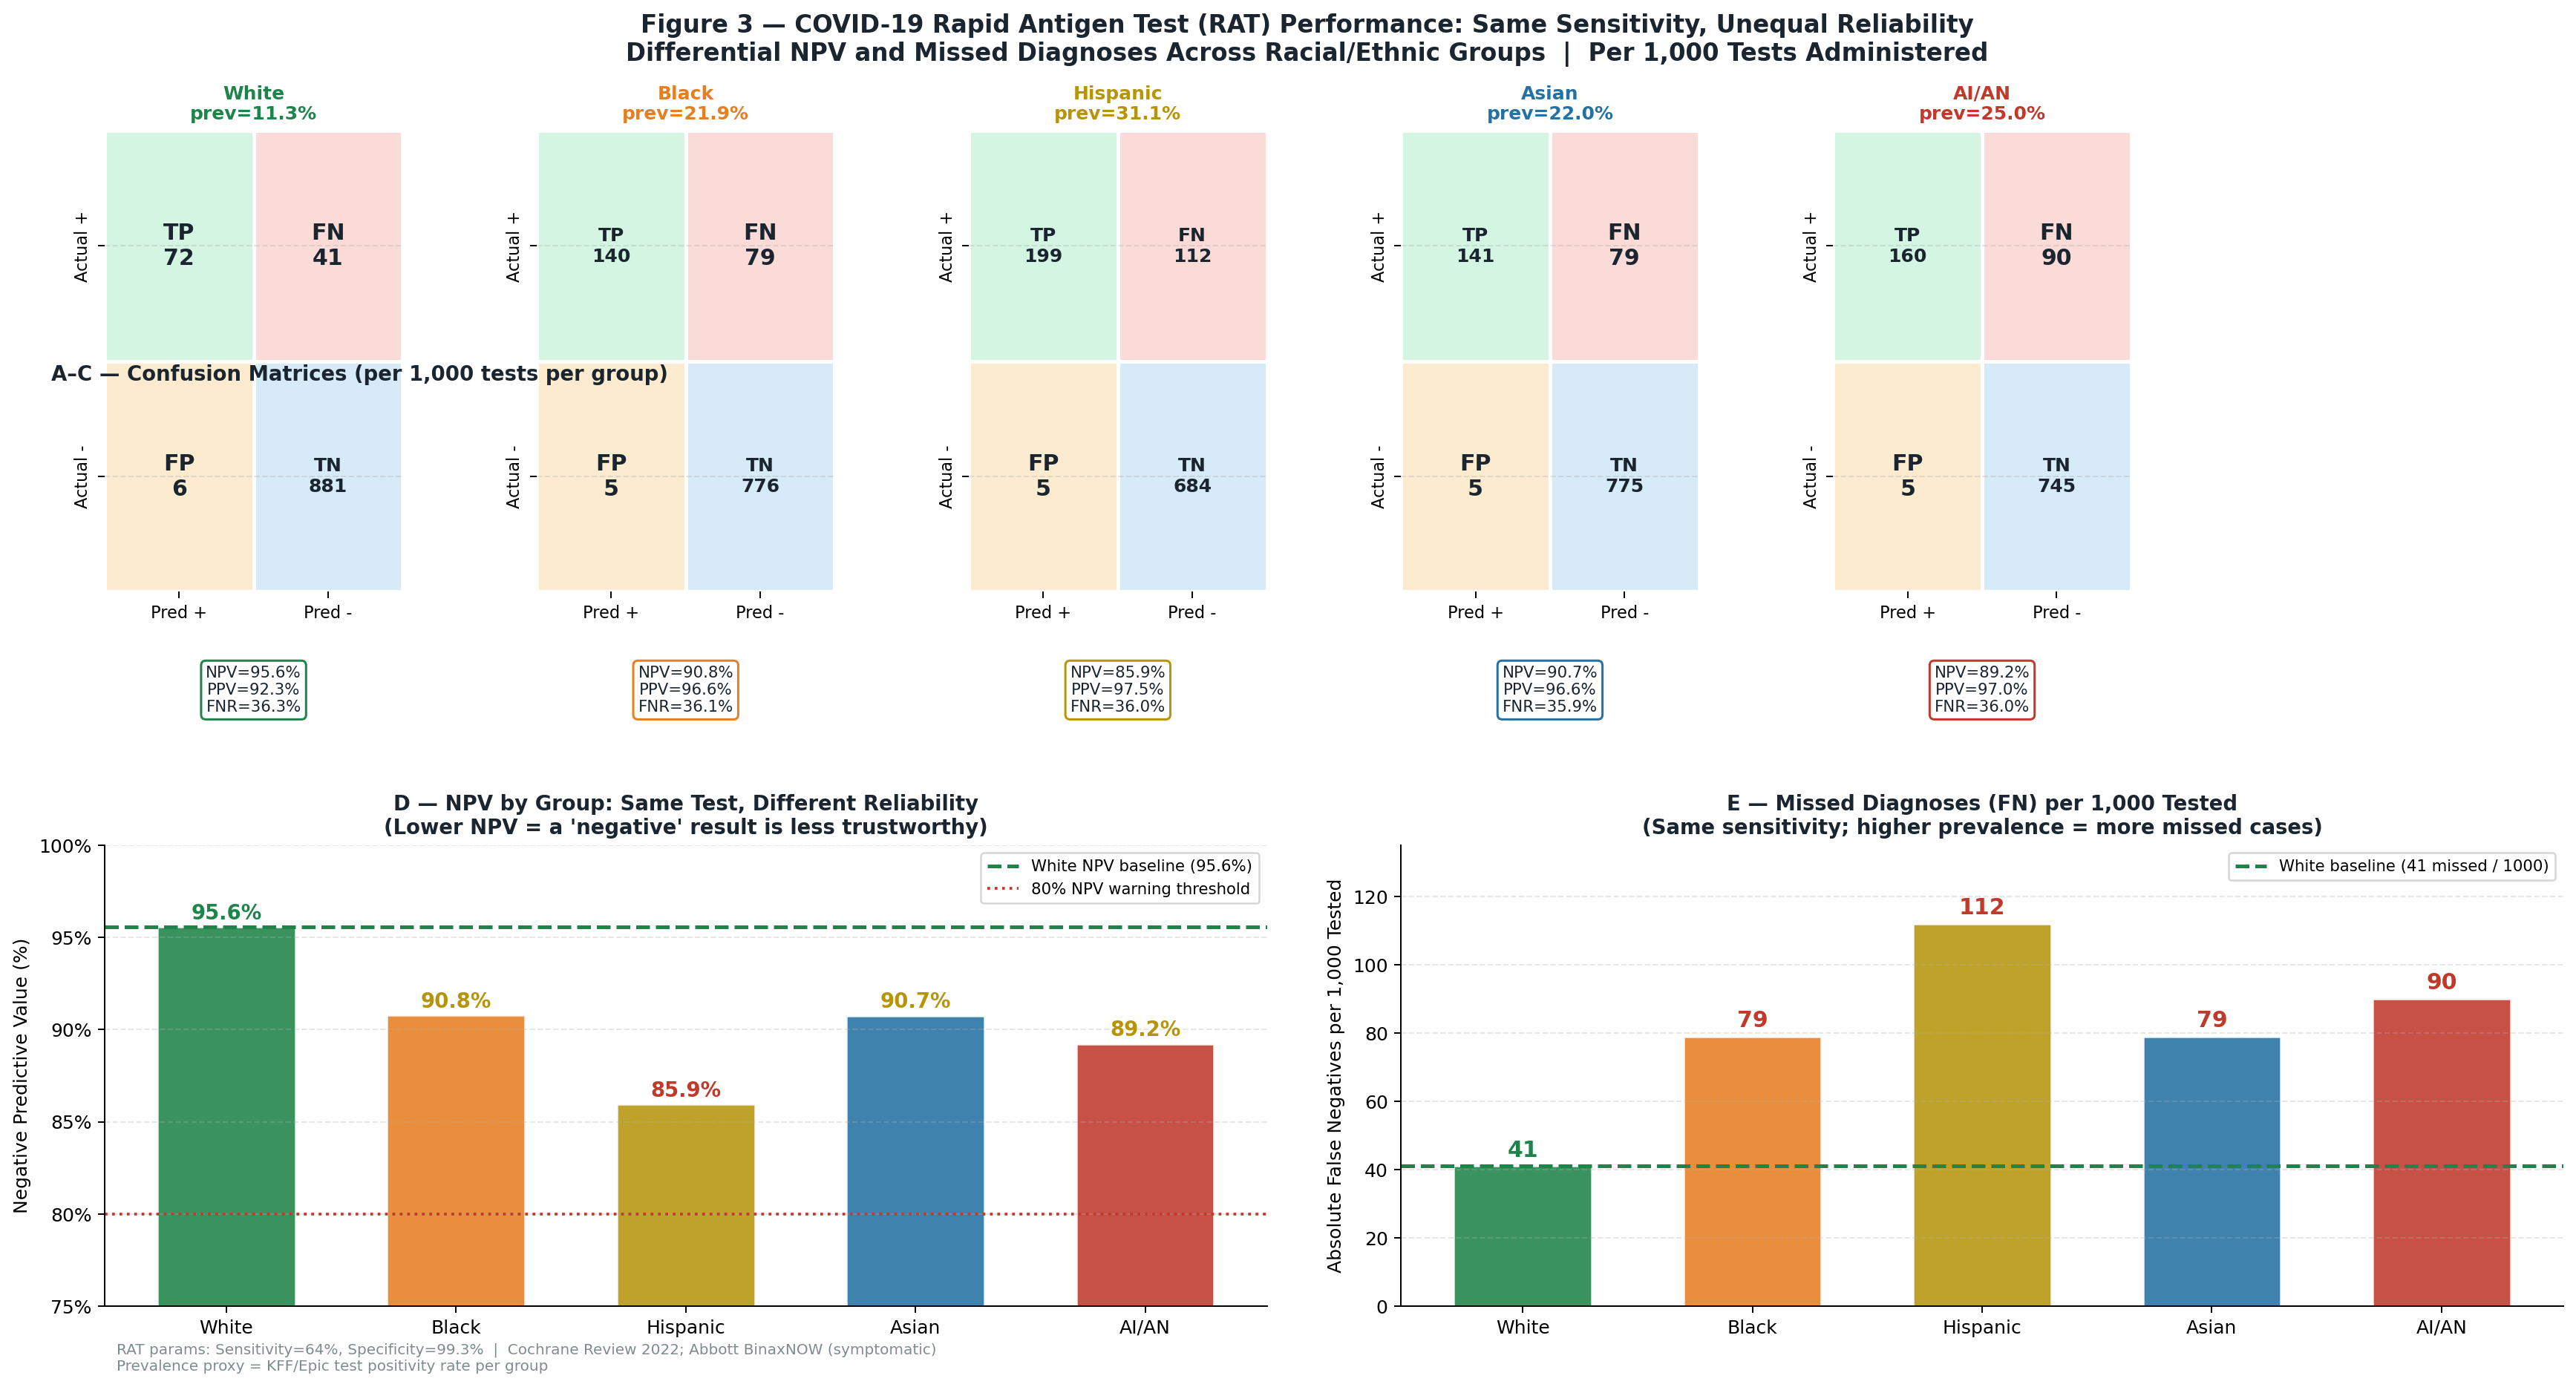
\includegraphics[width=\textwidth,height=0.68\textheight,keepaspectratio]{analysis_artifacts/fig3_confusion_matrices.png}}{%
\IfFileExists{analysis_artifacts/graph3_confusion_matrices.png}{\includegraphics[width=\textwidth,height=0.68\textheight,keepaspectratio]{analysis_artifacts/graph3_confusion_matrices.png}}{%
\IfFileExists{analysis_artifacts/graph3_confusion_matrix_routing.png}{\includegraphics[width=\textwidth,height=0.68\textheight,keepaspectratio]{analysis_artifacts/graph3_confusion_matrix_routing.png}}{%
\IfFileExists{analysis_artifacts/graph4_confusion_matrix_diagnostics.png}{\includegraphics[width=\textwidth,height=0.68\textheight,keepaspectratio]{analysis_artifacts/graph4_confusion_matrix_diagnostics.png}}{%
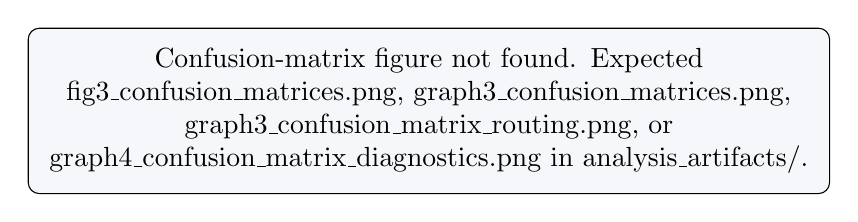
\begin{tikzpicture}\node[draw,rounded corners,fill=softgray,text width=0.82\textwidth,align=center,minimum height=2.1cm]{Confusion-matrix figure not found. Expected fig3\_confusion\_matrices.png, graph3\_confusion\_matrices.png, graph3\_confusion\_matrix\_routing.png, or graph4\_confusion\_matrix\_diagnostics.png in analysis\_artifacts/.};\end{tikzpicture}}}}}}

\begin{document}

\begin{frame}
  \titlepage
\end{frame}

\begin{frame}{Presentation Plan}
\begin{enumerate}
    \item Project overview and why missing context matters.
    \item Updated domain model.
    \item COVID clinical evidence: routing failure and diagnostic unreliability.
    \item Updated architecture and layer-by-layer implementation.
    \item GitHub code review and working demo plan.
    \item Next-semester completion plan.
\end{enumerate}
\begin{block}{Rubric target}
A clear 15-minute final presentation with quality figures, background that a common listener can follow, an updated domain model, updated architecture, code review, and demo path.
\end{block}
\end{frame}

\begin{frame}{Project Overview}
\begin{block}{Core problem}
Many applied data science systems are \textbf{sequential decision systems}: they route scarce resources under uncertainty, observe only partial feedback, and update future decisions from incomplete evidence.
\end{block}
\begin{columns}[T]
\begin{column}{0.48\textwidth}
\textbf{Clinical routing}
\begin{itemize}
    \item diagnostic tests and retests
    \item triage escalation
    \item model-assisted prioritization
    \item scarce attention during volatile conditions
\end{itemize}
\end{column}
\begin{column}{0.48\textwidth}
\textbf{Quantum routing}
\begin{itemize}
    \item route selection
    \item qubit allocation
    \item entanglement-generation effort
    \item noisy and non-stationary links
\end{itemize}
\end{column}
\end{columns}
\vspace{0.4em}
\alert{Goal:} compare performance and fairness across non-contextual, contextual, and informative contextual bandit policies.
\end{frame}

\begin{frame}{Why This Became a Clinical Fairness Problem}
\begin{block}{Missing context is not harmless}
A policy optimized only for aggregate reward can hide subgroup errors and compound disparities when one group has delayed testing, incomplete history, lower-quality measurements, or less representative calibration data.
\end{block}
\begin{center}
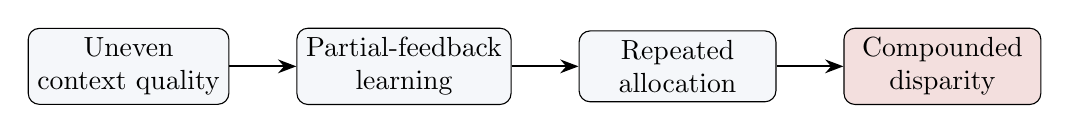
\begin{tikzpicture}[node distance=0.95cm, every node/.style={align=center}]
\node[draw, rounded corners, fill=softgray, minimum width=2.5cm, minimum height=0.75cm] (ctx) {Uneven\\context quality};
\node[draw, rounded corners, fill=softgray, right=0.85cm of ctx, minimum width=2.5cm, minimum height=0.75cm] (learn) {Partial-feedback\\learning};
\node[draw, rounded corners, fill=softgray, right=0.85cm of learn, minimum width=2.5cm, minimum height=0.75cm] (alloc) {Repeated\\allocation};
\node[draw, rounded corners, fill=softred!18, right=0.85cm of alloc, minimum width=2.5cm, minimum height=0.75cm] (harm) {Compounded\\disparity};
\draw[-{Stealth}, thick] (ctx) -- (learn);
\draw[-{Stealth}, thick] (learn) -- (alloc);
\draw[-{Stealth}, thick] (alloc) -- (harm);
\end{tikzpicture}
\end{center}
\vspace{0.3em}
\textbf{Clinical validation:} COVID test allocation and diagnostic validation both failed when critical group context was missing or ignored.
\end{frame}

\begin{frame}{Updated Domain Model}
\begin{center}
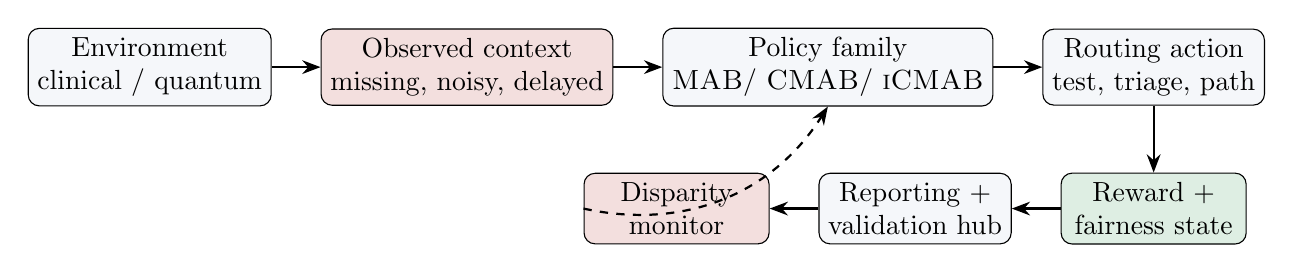
\begin{tikzpicture}[
  node distance=0.9cm,
  box/.style={draw, rounded corners, align=center, minimum width=2.35cm, minimum height=0.75cm, fill=softgray},
  bad/.style={draw, rounded corners, align=center, minimum width=2.35cm, minimum height=0.75cm, fill=softred!18},
  good/.style={draw, rounded corners, align=center, minimum width=2.35cm, minimum height=0.75cm, fill=softgreen!18},
  arr/.style={-{Stealth}, thick}
]
\node[box] (env) {Environment\\clinical / quantum};
\node[bad, right=0.62cm of env] (ctx) {Observed context\\missing, noisy, delayed};
\node[box, right=0.62cm of ctx] (policy) {Policy family\\\mab / \cmab / \icmab};
\node[box, right=0.62cm of policy] (action) {Routing action\\test, triage, path};
\node[good, below=0.85cm of action] (outcome) {Reward +\\fairness state};
\node[box, left=0.62cm of outcome] (report) {Reporting +\\validation hub};
\node[bad, left=0.62cm of report] (harm) {Disparity\\monitor};
\draw[arr] (env) -- (ctx);
\draw[arr] (ctx) -- (policy);
\draw[arr] (policy) -- (action);
\draw[arr] (action) -- (outcome);
\draw[arr] (outcome) -- (report);
\draw[arr] (report) -- (harm);
\draw[arr, dashed] (harm.west) to[bend right=35] (policy.south);
\end{tikzpicture}
\end{center}
\begin{itemize}
    \item One environment produces many contexts; one policy selects one action per round.
    \item One action produces one observed reward, while unchosen actions remain counterfactual.
    \item Fairness risk appears when context quality is worse for one group, site, cohort, flow, or route class.
\end{itemize}
\end{frame}

\begin{frame}{Best Evidence Figure 1: Test Routing Failure vs. CMAB Routing}
\begin{center}
\routingfig
\end{center}
\vspace{-0.2em}
\small \textbf{Finding:} context-blind routing detects 17.2 cases per 100 tests, while context-aware CMAB routing detects 19.3 cases per 100 tests, a 12.5\% efficiency gain while increasing allocation to AIAN, Black, and Hispanic groups.
\end{frame}

\begin{frame}{What Figure 1 Means for the Research}
\begin{columns}[T]
\begin{column}{0.48\textwidth}
\textbf{Context-blind allocation}
\begin{itemize}
    \item White non-Hispanic group receives 61.5\% of tests.
    \item This group has the lowest positivity rate: 11.3\%.
    \item High-vulnerability groups remain under-served.
\end{itemize}
\end{column}
\begin{column}{0.48\textwidth}
\textbf{CMAB-aware allocation}
\begin{itemize}
    \item Weights allocation by vulnerability and hospitalization context.
    \item AIAN: 2.4$\times$, Black: 2.0$\times$, Hispanic: 1.8$\times$ hospitalization context.
    \item Routes scarce tests toward higher-yield and higher-risk groups.
\end{itemize}
\end{column}
\end{columns}
\begin{block}{Slide message}
Fairness and efficiency are not opposites here. Better context improves both equity and case-finding yield.
\end{block}
\end{frame}

\begin{frame}{Best Evidence Figure 2: Missing Minority Context in Diagnostics}
\begin{center}
\diagnosticfig
\end{center}
\vspace{-0.2em}
\small \textbf{Finding:} the groups with higher COVID mortality and positivity were also less represented in diagnostic-validation evidence; Black participants appear at 53.7\% of expected representation in prevention/diagnostic trials.
\end{frame}

\begin{frame}{What Figure 2 Means for the Research}
\begin{columns}[T]
\begin{column}{0.50\textwidth}
\textbf{Trial and testing signal}
\begin{itemize}
    \item Black participants: 53.7\% of expected representation.
    \item White participants: 110\% of expected representation.
    \item Hispanic positivity: 31.1\%; Black positivity: 21.9\%.
\end{itemize}
\end{column}
\begin{column}{0.46\textwidth}
\textbf{Bandit interpretation}
\begin{itemize}
    \item The reward signal is cleaner for well-measured groups.
    \item The policy can learn confidence for the wrong population.
    \item EQUITAS-style context monitoring makes the reliability gap visible.
\end{itemize}
\end{column}
\end{columns}
\begin{block}{Slide message}
Missing group context creates a diagnostic reliability problem before the bandit ever chooses an action.
\end{block}
\end{frame}

\begin{frame}{Best Evidence Figure 3: Confusion-Matrix Findings}
\begin{center}
\confusionfig
\end{center}
\vspace{-0.2em}
\small \textbf{Finding:} the same diagnostic policy can produce different false-negative and NPV behavior across groups when prevalence and validation representation differ.
\end{frame}

\begin{frame}{Confusion-Matrix Interpretation}
\begin{columns}[T]
\begin{column}{0.48\textwidth}
\textbf{Routing matrix}
\begin{itemize}
    \item Context-blind routing wastes capacity on lower-yield groups.
    \item CMAB-aware routing improves cases detected from the same test supply.
    \item The key metric is cases detected per 100 tests plus group disparity.
\end{itemize}
\end{column}
\begin{column}{0.48\textwidth}
\textbf{Diagnostic matrix}
\begin{itemize}
    \item Under-representation creates poorer test reliability for some groups.
    \item Group-level NPV/FNR monitoring is required.
    \item EQUITAS mediation flags groups where a negative result is least trustworthy.
\end{itemize}
\end{column}
\end{columns}
\begin{block}{Slide message}
A single aggregate accuracy score is not enough; the matrix must be stratified by context group.
\end{block}
\end{frame}

\begin{frame}{Updated Architecture Overview}
\begin{center}
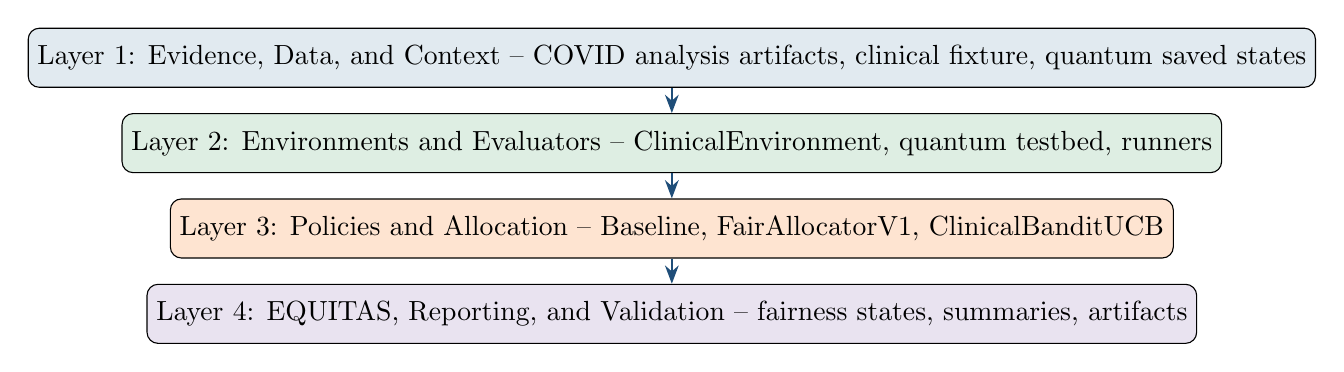
\begin{tikzpicture}[
  layer/.style={draw, rounded corners, align=center, minimum width=10.2cm, minimum height=0.75cm, fill=softgray},
  arr/.style={-{Stealth}, thick, deepblue}
]
\node[layer, fill=softblue!18] (data) {Layer 1: Evidence, Data, and Context -- COVID analysis artifacts, clinical fixture, quantum saved states};
\node[layer, fill=softgreen!18, below=0.32cm of data] (env) {Layer 2: Environments and Evaluators -- ClinicalEnvironment, quantum testbed, runners};
\node[layer, fill=ritorange!18, below=0.32cm of env] (policy) {Layer 3: Policies and Allocation -- Baseline, FairAllocatorV1, ClinicalBanditUCB};
\node[layer, fill=softpurple!18, below=0.32cm of policy] (report) {Layer 4: EQUITAS, Reporting, and Validation -- fairness states, summaries, artifacts};
\draw[arr] (data) -- (env);
\draw[arr] (env) -- (policy);
\draw[arr] (policy) -- (report);
\end{tikzpicture}
\end{center}
\begin{block}{Design principle}
Low coupling: each layer exposes records/artifacts to the next layer. High cohesion: each layer has one job: context, environment, decision, or validation.
\end{block}
\end{frame}

\begin{frame}{Architecture Layer 1: Evidence, Data, and Context}
\begin{columns}[T]
\begin{column}{0.48\textwidth}
\textbf{Inputs}
\begin{itemize}
    \item COVID clinical evidence artifacts
    \item clinical synthetic fixture
    \item EQUITAS context fields
    \item quantum legacy saved states
\end{itemize}
\end{column}
\begin{column}{0.48\textwidth}
\textbf{Context fields}
\begin{itemize}
    \item group, site, cohort, service line
    \item test distribution and escalation action
    \item reward, success, latency
    \item route choice, allocator, evaluator state
\end{itemize}
\end{column}
\end{columns}
\begin{block}{Why this layer matters}
The new artifacts make the clinical side evidence-based: vulnerability, representation, and measurement quality must be modeled before a fair policy can act.
\end{block}
\end{frame}

\begin{frame}{Architecture Layer 2: Environments and Evaluators}
\begin{columns}[T]
\begin{column}{0.48\textwidth}
\textbf{Clinical path}
\begin{itemize}
    \item \texttt{ClinicalEnvironment}
    \item \texttt{ClinicalExperimentRunner}
    \item \texttt{ClinicalExperimentEvaluator}
    \item synthetic clinical allocation fixture
\end{itemize}
\end{column}
\begin{column}{0.48\textwidth}
\textbf{Quantum path}
\begin{itemize}
    \item quantum-routing testbed
    \item evaluator and saved-state conventions
    \item fairness sidecar artifacts
    \item compatibility with legacy experiments
\end{itemize}
\end{column}
\end{columns}
\begin{block}{Layer relationship}
The evaluator standardizes outcome records so clinical and quantum runs can be compared through the same reporting and validation surface.
\end{block}
\end{frame}

\begin{frame}{Architecture Layer 3: Policies and Allocation}
\begin{center}
\begin{tabular}{p{0.24\textwidth}p{0.28\textwidth}p{0.35\textwidth}}
\toprule
Policy family & Decision signal & Fairness risk \\
\midrule
\mab & action history only & repeats historical allocation patterns \\
\cmab & observed context & improves utility but can inherit incomplete context \\
\icmab & context + fairness state & tests whether mediated context reduces harm \\
\bottomrule
\end{tabular}
\end{center}
\begin{block}{Clinical model families used in smoke validation}
Oracle, ClinicalBaseline, FairAllocatorV1, and ClinicalBanditUCB.
\end{block}
\begin{equation*}
\text{decision}_t = \arg\max_a \left[\text{utility}_{t,a} - \lambda \cdot \text{expected disparity}_{t,a}\right]
\end{equation*}
\end{frame}

\begin{frame}{Architecture Layer 4: EQUITAS, Reporting, and Validation}
\begin{columns}[T]
\begin{column}{0.48\textwidth}
\textbf{EQUITAS mediation}
\begin{itemize}
    \item attaches audit/mitigation context
    \item tracks group-conditioned outcomes
    \item separates artifact validation from unvalidated active quantum updates
\end{itemize}
\end{column}
\begin{column}{0.48\textwidth}
\textbf{Reporting layer}
\begin{itemize}
    \item model-stratified fairness summaries
    \item manifest-linked report artifacts
    \item validation hub checks evidence claims
\end{itemize}
\end{column}
\end{columns}
\begin{block}{Preliminary framework validation}
The clinical fairness smoke produced 16 fairness states; report generation produced 21 manifest-linked artifacts.
\end{block}
\end{frame}

\begin{frame}{Preliminary Framework Results}
\begin{center}
\begin{tabular}{p{0.43\textwidth}p{0.42\textwidth}}
\toprule
Evidence item & Result \\
\midrule
Clinical embedded path & evaluator, runner, environment, allocator, models, and EQUITAS context run end-to-end \\
Clinical fairness smoke & 16 fairness states across four model families \\
Non-oracle efficiency & FairAllocatorV1: 91.23\%; ClinicalBanditUCB: 84.21\%; ClinicalBaseline: 75.09\% oracle efficiency \\
Reporting layer & 21 manifest-linked artifacts and model-stratified summaries \\
Quantum compatibility & legacy quantum path preserved with fairness sidecar artifacts \\
\bottomrule
\end{tabular}
\end{center}
\small Boundary: active fairness-adjusted quantum learning still requires an explicit policy-update mechanism and full validation.
\end{frame}

\begin{frame}{GitHub Code Review Break}
\begin{block}{Show 2--3 classes not used in the midterm}
During the live code break, open GitHub and connect each class to the architecture diagram.
\end{block}
\begin{center}
\small
\begin{tabular}{p{0.34\textwidth}p{0.48\textwidth}}
\toprule
Class / file to show & Architecture connection \\
\midrule
\texttt{ClinicalExperimentEvaluator} & Layer 2 evaluator orchestration and artifact capture \\
\texttt{ClinicalExperimentRunner} & Layer 2 run execution over seeds, models, and allocations \\
\texttt{FairAllocatorV1} or \texttt{ClinicalBanditUCB} & Layer 3 policy/allocation decision logic \\
\texttt{equitas\_mediator.py} & Layer 4 fairness audit and mitigation context \\
\bottomrule
\end{tabular}
\end{center}
\small Mention comments, formatting, and how the classes expose low coupling/high cohesion across layers.
\end{frame}

\begin{frame}{Working Demo Plan}
\begin{enumerate}
    \item Run the clinical fairness demo or smoke validation notebook.
    \item Show generated fairness states and model-stratified summaries.
    \item Show report artifacts and manifest linkage.
    \item Open the validation hub and point to the five validated evidence claims.
    \item Show how the new COVID clinical artifacts become next-semester executable environments.
\end{enumerate}
\begin{block}{Demo objective}
Show that the system runs, records fairness evidence, and produces artifacts connected to the architecture.
\end{block}
\end{frame}

\begin{frame}{Next Semester: Architecture Completion}
\begin{enumerate}
    \item Convert COVID test allocation and diagnostic-bias evidence into executable clinical environments.
    \item Add the best analysis artifacts into the final paper and reporting pipeline.
    \item Complete active fairness-adjusted quantum policy updates.
    \item Split validation into efficiency and fairness hubs.
    \item Build a reporting layer that links framework outputs, validation evidence, and paper claims.
\end{enumerate}
\begin{block}{Longer-term goal}
A portal-style reporting surface for queries, experiments, validation, and paper-ready evidence.
\end{block}
\end{frame}

\begin{frame}{Takeaway}
\begin{block}{Main scientific claim}
Context quality is a fairness variable. Missing, ignored, or biased context can turn partial-feedback learning into repeated allocation harm.
\end{block}
\begin{block}{What was built}
A clinical--quantum evaluation framework that compares performance and fairness across the selected MAB spectrum while preserving reproducible artifacts.
\end{block}
\begin{block}{What the new analysis adds}
The analysis artifacts provide clinical evidence that validates the missing-context harm model: test routing improved by context-aware allocation, and diagnostic reliability changed when group context was missing.
\end{block}
\end{frame}

\begin{frame}[allowframebreaks]{Selected References}
\scriptsize
\begin{thebibliography}{99}
\bibitem{kffepic} KFF/Epic. COVID-19 racial disparities in testing, infection, hospitalization, and death.
\bibitem{cdcdisparities} CDC. Risk for COVID-19 infection, hospitalization, and death by race/ethnicity.
\bibitem{mody2021} Mody et al. Racial and ethnic disparities in COVID-19 testing and outcomes. \textit{Clinical Infectious Diseases}, 2021.
\bibitem{dalvabaird2021} Dalva-Baird et al. Racial and ethnic inequities in the early distribution of U.S. COVID-19 testing sites. 2021.
\bibitem{trials2022} Systematic review/meta-analysis of racial and ethnic representation in U.S. COVID-19 trials.
\bibitem{garcia2026} Garcia Bautista. DSCI601 project proposal, rough report, architecture, and fairness framework materials.
\end{thebibliography}
\end{frame}

\end{document}
